\documentclass[11pt]{report}
\usepackage{amsmath,amsthm,amssymb,wasysym}
\usepackage{mathtools}
\usepackage{enumerate}
\usepackage{graphicx}
\usepackage{mathpazo}
\usepackage{lmodern}
\usepackage{parskip}
\usepackage{fancyhdr}
\usepackage{wrapfig}
\usepackage{tikz}
\usepackage{hyperref}
\usepackage{listings}
\lstdefinestyle{MyPythonStyle}
{
    language=Python,
    basicstyle=\footnotesize,
    numbers=left,
    stepnumber=1,
    showstringspaces=false,
    tabsize=1,
    breaklines=true,
    breakatwhitespace=false,
}
\lstdefinestyle{MyCStyle}
{
    language=[Sharp]C,
    basicstyle=\footnotesize,
    numbers=left,
    stepnumber=1,
    showstringspaces=false,
    tabsize=1,
    breaklines=true,
    breakatwhitespace=false,
}
\usepackage[linesnumbered,algoruled,boxed,lined]{algorithm2e}
\usetikzlibrary{positioning, shapes.geometric, arrows}
\tikzstyle{startstop} = [rectangle, rounded corners, text centered, draw=black, fill=red!30]
\tikzstyle{io} = [text centered]
\tikzstyle{decision} = [rectangle, text centered, draw=black]
\tikzstyle{process} = [trapezium, text centered, draw=black]
\tikzstyle{arrow} = [thick,->,>=stealth]
\newtheorem{theorem}{Theorem}
\newtheorem{defn}{Definition}
\newcommand{\Jostle}{\texttt{Jostle}}
\newcommand{\dbspace}{\mathcal{R}}
\newcommand{\featspace}{\mathcal{X}}
\renewcommand{\t}[1]{\texttt{#1}}
\lhead{Senior Thesis}
\rhead{Jacob Imola}
\cfoot{\thepage}
\pagestyle{fancy}
\title{Automatic, Fine-Grained Algorithmic Choice for Differential Privacy}
\date{\today}
\author{Jacob Imola\\ School of Computer Science, Carnegie Mellon University\and Jean Yang\\ School of Computer Science, Carnegie Mellon University}
\begin{document}
\maketitle
\chapter{Introduction}\label{ch:intro}
The rapid technological increase in data collection, speed, and storage has brought about revolutionary insights and ideas and will continue to do so. However, with huge amounts of private data comes the concern of preventing data from ending up in the wrong hands. In order to prevent data leakage, we must lay a strong privacy foundation and give data programmers tools for implementing privacy both efficiently and correctly.

Consider a healthcare database with records like patient weight, age, genetic information, and whether they are HIV positive. Granting access rights, or policies, to just patients and their doctors protects as much privacy as possible, and developing tools for verifying information flow policies is an interesting question in its own right that has been studied immensely. However, sometimes it's okay to release some statistics about the database so that a programmer can find risk factors for people who have HIV. Publicly releasing the entire database doesn't protect privacy at all, yet it would be a programmer's dream. In order to appease both data programmers and patients, a middle ground area must be chosen where a blurry snapshot of the database is released, comprehensive enough so that meaningful conclusions may be drawn yet blurry enough so that individuals are mostly protected. We call this the \emph{privacy-accuracy} tradeoff. We can always sacrifice one for the other before we disclose our database snapshot. However, after we disclose, it is impossible to take any privacy back, so we have to be absolutely sure that privacy guarantee will not fail under any attack. The most promising method for doing such a disclosure is Differential Privacy~\cite{Dwork:2006}.

Differential Privacy (DP) is considered to be the gold-standard of privacy and has been researched intensely since its conception in 2005. Its goal is to provide guarantees on what can be done with the information being released from a dataset while making minimal assumptions about an attacker's abilities. Previous attempts at privacy were susceptible to surprise exploits that occurred after a database was released. Notably, before DP, researchers were able to reidentify users in a Netflix dataset given an auxiliary dataset from IMDB and form a generalized attack against the state-of-the-art privacy algorithms of the time~\cite{Narayanan:2006}. The strong privacy guarantee of DP, on the other hand, has a rigorous mathematical foundation that makes it impervious to the post-processing attacks that compromised the Netflix dataset, and more recently, \href{https://hackernoon.com/how-to-rob-an-airbnb-252e7e7eda44}{AirBnB} and \href{https://gizmodo.com/this-is-almost-certainly-james-comey-s-twitter-account-1793843641}{Instagram}. Differential Privacy has stood the test of time as a sturdy way to protect privacy.

However, just building a suite of DP algorithms is not satisfactory. Differential Privacy necessarily adds randomness to programs, and randomness adds a new layer of complexity to programs. For example, adding noise to a variable that governs how many times a loop is performed could result in two highly different program executions and thus a very noisy answer. However, in many DP applications, noise can be added in a number of places, different queries could be done to accomplish the same goal, and so on. A very noisy answer could potentially be avoided if the proper algorithm is deployed. If one algorithm always dominated the others, this wouldn't be much of a problem, but as we will see, the best one depends on the database in a complex way. Picking the best algorithm for the job depends on extensive empirical evaluations, as theoretical bounds are often insufficient for complex algorithms~\cite{Hay:2016}. This leads the central problem addressed by this work:

\textbf{Problem:} How can we alleviate the burden of empirical algorithmic choice from the programmer? 

This problem is noted by the authors of DPComp~\cite{Hay:2016}, who comment that currently, ``the practitioner is lost and incapable of deploying the right algorithm''. DPComp allows the programmer to visualize the performances of different histogram querying algorithms on certain datasets. An example of one algorithm executed on one dataset is shown in Figure~\ref{fig:dpcomp}. We feel this is a step in the right direction, but their approach would be better if its ideas were applied to a programming language. The approach is to move the manual exploration of algorithms that a programmer might do with DPComp into the runtime of our programming language, which we call \Jostle{}, so named because it will ``jostle'' the various algorithms during runtime. This will give the following benefits:

\begin{figure}
\begin{center}
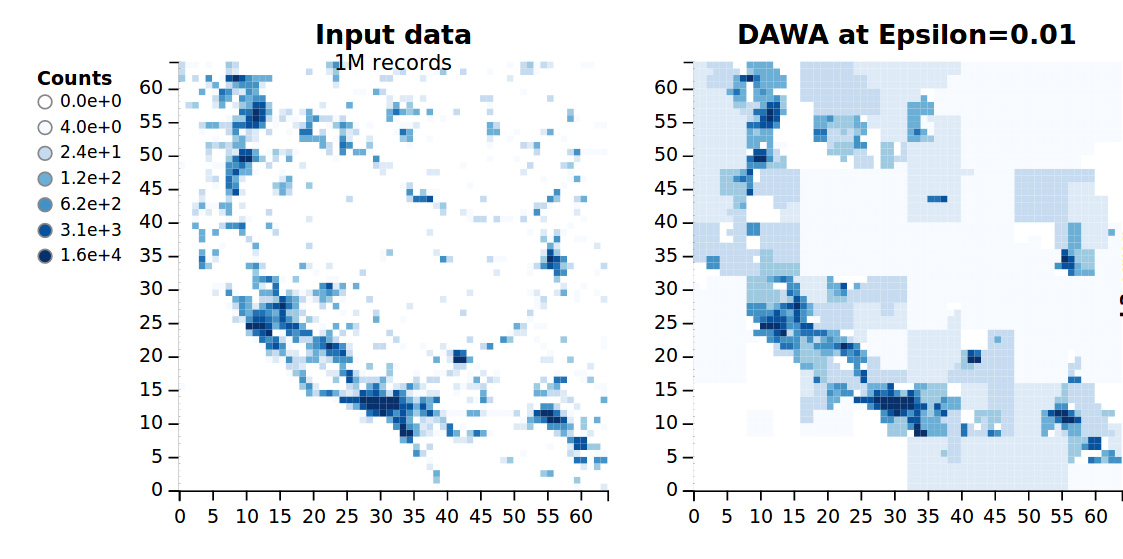
\includegraphics[scale=0.3]{DPComp}
\end{center}
\caption{A screenshot of a DPComp graph depicting the original dataset and the noise that a DP algorthm, DAWA~\cite{Li:2014}, adds at $\epsilon=0.01$. This would help a programmer decide whether to apply DAWA on his own dataset.}\label{fig:dpcomp}
\end{figure}
\begin{enumerate}
\item \textbf{Correctness} A \Jostle{} program enjoys the DP correctness guarantees that existing DP programming languages give. Correctness in the area of privacy is particularly important because privacy breaches are costly.
\label{itm:adv_correct}
\item \textbf{Generalization} The DPComp study of 2D histograms does not easily generalize to other DP algorithms. A programming language is far more general as arbitrary code can be analyzed. Concretely, DPComp can be implemented as a specific \Jostle{} program, and not the other way round.
\label{itm:adv_general}
\item \textbf{Differential Privacy Insight} DPComp is also a teaching tool because it advances one's knowledge of how algorithms perform on datasets. Every time a \Jostle{} program picks a algorithm, its trace extends a programmer's understanding of performance improves. This insight is particularly helpful to programmers new to DP who have no clues as to which algorithm to deploy.
\label{itm:adv_insight}
\end{enumerate}

Even though programming languages exist which confer benefit \ref{itm:adv_correct} and DPComp confers benefits \ref{itm:adv_general} and \ref{itm:adv_insight}, no works enjoy all three benefits at the same time. Having all three benefits is important because of programmer burden. Doing a DPComp-style analysis every time algorithmic choice needs to be explored requires doing data analysis on all algorithms and then implementing the insights by hand. Once algorithms are implemented, there is a small overhead writing \Jostle{} code to make the choice. The algorithmic insights come for free via the \Jostle{} trace.

\Jostle{} will represent algorithmic choice with the \t{MakeChoice} statement, illustrated in Figure~\ref{fig:1}.
\begin{figure}
\begin{lstlisting}[style=MyCStyle]
trainingSet = {US Census, ... #Public Databases}

uniformity = Metafeature(data){
    db = data.database
    xgrp = sqrt(db.x_range)
    ygrp = sqrt(db.y_range)
    return {{stddev(select sum(values) from db 
                    groupby x/xgrp, y/ygrp)}}
}
sparsity = Metafeature(data){
    db = data.database
    num_nonzero = {{select count(values) from db 
                    where values > 0}}
    domain_size = db.x_range * db.y_range
    return num_nonzero/domain_size
}

DAWA = Option(data){
    //DAWA Implementation
}
MWEM = Option(data){
    //MWEM Implementation
}

scoreFunc = Utility(data, answers){
    //compare answers to data.queries run on non-private data.answers
}

noisyHistChoice = MkChoiceMaker among {DAWA, MWEM}
                    informed by {uniformity, sparsity}
                    trained on trainingSet 
                    wrt ScoreFunc
def answerHistQueries(data):
    answers = noisyHistChoice(data)
\end{lstlisting}

\caption{\Jostle{} code demonstrating the use of \t{ChoiceMaker} object, called \t{noisyHistChoice}. In this case, the options are the \t{DAWA} and \t{MWEM} 2D Histogram algorithms.}
\label{fig:1}
\end{figure}
A programmer will use a \t{ChoiceMaker} when they are unsure of which choice to make at a certain point in their code; in the example, they are choosing between the algorithms \t{DAWA}~\cite{Li:2014} and \t{MWEM}~\cite{Hardt:2010}. The constructor, \t{MkChoiceMaker}, takes in a set of \t{Options}, a set of training databases, and a set of functions from the database to $\mathbb{R}$ called metafeatures.

The above design is inspired by DPComp. Suppose we are a programmer deciding whether to run the \t{DAWA} algorithm on a public dataset shown in Figure~\ref{fig:dpcomp}. We may notice that the input is a rather sparse and non-uniform---most of the points are 0 (white) and the non-zero points are clustered into groups. Indeed, this dataset is the population distribution for the southwest United States. We decide that these two properties adversely affect the performance for \t{DAWA}, as it predicts many of the white points incorrectly to have a nonzero value. Similarly, \t{sparsity} might affect the performance of \t{MWEM}, but not \t{uniformity}. The set of all properties that may impact performance are the \emph{metafeatures}. They are database properties that we pay attention to when we estimate algorithm performance.

\t{MkChoiceMaker} will train a model from the set of metafeatures to predicted algorithm performance. The resulting \t{ChoiceMaker} can be called on a private database. When this happens, the metafeatures are evaluated on the database and the \t{Option} with the highest estimated performance is dispatched.

We will begin with a background section on DP and related work. Then, we will present a formal outline of how \Jostle{} runs. Thirdly, we will implement Decision Tree choice with \Jostle{} and provide empirical evidence for the claimed benefits (Page~\pageref{itm:adv_correct}) of \Jostle{}. Finally, we will discuss future directions for \Jostle{}.

\chapter{Background}\label{ch:background}
\section{Differential Privacy}
Differential Privacy makes the following promise to data subjects: ``You will not be affected, adversely or otherwise, by allowing your data to be used in any study or analysis, no matter what other studies, data sets, or information sources, are available''~\cite{Dwork:2006}. To make this more formal, we must analyze two databases, $D$ and $D'$, differing in only one row which represents a database before and after a user participates. We call such databases neighbors. Suppose we are running a algorithm $\mathcal{M}$ on the database. If an attacker is able to discern with confidence $\mathcal{M}(D)$ and $\mathcal{M}(D')$, then this poses a privacy threat. The strength of this confidence is quantified a real number $\epsilon$ such that small $\epsilon$ corresponds to low attacker confidence. This means that deterministic algorithms are already unacceptable if it's possible for $\mathcal{M}(D) \neq \mathcal{M}(D')$. We necessarily must output a probability distribution, and once we view $\mathcal{M})(D)$ as a distribution, we can finally pin down the definition:

\begin{defn}
$\mathcal{A}$ satisfies $\epsilon$-DP if for all $D$ and $D'$ such that $|D-D'|_1=1$ and for all $o$ in the range of $\mathcal{M}$, 
\[\Pr\left(\mathcal{M}(D) = o \right) \leq e^{\epsilon} \Pr\left(\mathcal{M}(D')=o\right)\]
\end{defn}

There is also a more general definition that gives a weaker privacy guarantee: 

\begin{defn}
$\mathcal{M}$ satisfies $(\epsilon, \delta)$-DP if for all $D$ and $D'$ such that $|D-D'|_1=1$ and for all $o$ in the range of $\mathcal{M}$, 
\[\Pr\left(\mathcal{A}(D) = o \right) \leq e^{\epsilon} \Pr\left(\mathcal{M}(D')=o \right) + \delta\]
\end{defn}

For much of this paper, we will focus on $\epsilon$-DP, but it is worth knowing the more general case so we can import the well-known privacy theorems in their full generality.

The definition doesn't address why the ``no matter what'' part of the promise is true, but we can view any post-release attack on $\mathcal{A}$ as a function $F$ that doesn't involve $D$. Then, the following theorem establishes the promise:

\begin{theorem}
(Post-Processing~\cite{Dwork:2006}) If $\mathcal{M}$ satisfies $(\epsilon, \delta)$-DP, and $F$ is any function that takes the output of $\mathcal{M}$ as input, then $F(\mathcal{M})$ satisfies $(\epsilon, \delta)$-DP.
\end{theorem}
This theorem is the reason why DP is such a useful guarantee. Data programmers can be sure that once they run their algorithm $\mathcal{M}$ and release its output, then the DP guarantee gets no weaker \emph{no matter what an adversary does with the data}. This prevents the headaches where a programmer realizes retroactively that the data he released can be combined in some way to reveal much more information than was intended, like in Netflix~\cite{Narayanan:2006}.

In addition, DP satisfies several other useful properties:

\begin{theorem} \label{thm:comp}
(Composition~\cite{Dwork:2006}) Given algorithm $M_1$ and $M_2$ satisfying $\epsilon_1$ and $\epsilon_2$ DP, respectively, along with a database $D$, the algorithm $M = (M_1(D), M_2(D))$ has $(\epsilon_1+\epsilon_2, \delta_1+\delta_2)$ DP.
\end{theorem}
Composition is like the union bound from probability; it's convenient to apply but often is a pessimistic bound, as we will see later. Because of composition, we often refer to $\epsilon$ as a privacy budget---if we string together many private computations, it's like we spend some of our budget on each one out of a total budget of $\epsilon$.

We can easily improve upon Composition in the special case of algorithms operating on disjoint parts of the database. If $D$ is split into disjoint parts before algorithms are applied to it, then out of all its possible neighbors, only one of the parts will be different. Thus, only the worst algorithm will affect the DP guarantee:
\begin{theorem}\label{thm:disj}
(Disjointness~\cite{Dwork:2006}) Given disjoint subsets $D_1, D_2$ of $D$ with two algorithms $M_1$ and $M_2$ providing $(\epsilon_1, \delta_1)$ and $(\epsilon_2, \delta_2)$-privacy, then $((M_1(D_1), M_2(D_2))$ satisfies $(\max\{\epsilon_1, \epsilon_2\}, \max\{\delta_1, \delta_2\})$-DP.
\end{theorem}

So, what's a simple example of a DP algorithm? Suppose each row of our database $D$ is 0 or 1, so $D \in \{0, 1\}^n$, and that we are trying to release the sum of the elements of $D$. If this sum is $S$, then all neighboring databases $D'$ have sum $S$ or $S+1$. We can add noise to $S$ so that it looks very similar in distribution to $S+1$. The distribution we are looking for is the Laplace distribution:
\begin{defn}
The $\text{Laplace}(\lambda)$ distribution has probability mass function $f(x) = \frac{1}{2\lambda}e^{-|x|/\lambda}$.
\end{defn}
This distribution fits perfectly with the definition of DP because of the exponentials. If $X,Y$ are i.i.d. from $\text{Laplace}\left(\frac{1}{\epsilon}\right)$, then it is straightforward to show that the distributions of $S+X$ and $S+1+X$ satisfy $(\epsilon, 0)$ DP. To generalize this statement, we will use the following definition:
\begin{defn}
(Sensitivity) A function $f$ is $\Delta$-sensitive if for all $x,y$ such that $|x-y|_1 = 1$, we have 
\[
|f(x) - f(y)| \leq \Delta
\]
This can equivalently be rephrased as 
\[
\max_{|x-y|_1=1}|f(x) - f(y)| = \Delta
\]
We will denote the sensitivity of $f$ by $\Delta(f)$.
\end{defn}
This gives us the following algorithm:

\begin{algorithm}\label{alg:1}
\SetAlgoLined
\SetKwInOut{Input}{Input}\SetKwInOut{Output}{Output}
\Input{$D$, a database; $f$, a function $\mathcal{D} \rightarrow \mathbb{R}^n$; and $\epsilon$}
\Output{An estimate for $f(D)$ satisfying $\epsilon$-DP.}
$X$, a vector of $n$ i.i.d. variables drawn from $\text{Laplace}\left(\frac{\Delta(f)}{\epsilon}\right)$\;
\Return{X+f(D)}
\caption{Laplace Mechanism}
\end{algorithm}

\begin{theorem}
The Laplace mechanism~\ref{alg:1} satisfies $(\epsilon, 0)$-DP~\cite{Dwork:2006}.
\end{theorem}
For the counting or histogram queries such as our example above, we have $\Delta = 1$ so we add $\text{Laplace}\left(\frac{1}{\epsilon}\right)$ noise to our function.

However, what if we wanted to compute the maximum value in a set? If we had $n$ elements, we certainly wouldn't want to apply Composition $n$ times, obtaining $n\epsilon$-DP, just to have $\t{Laplace}\left(\frac{1}{\epsilon}\right)$ noise added to our answer. A better way is to use ReportNoisyMax~\ref{alg:max}. Instead of paying $n\epsilon$, ReportNoisyMax allows us to pay $\epsilon$ for the exact same noise on our answer.
\begin{algorithm}\label{alg:max}
\SetAlgoLined
\SetKwInOut{Input}{Input}\SetKwInOut{Output}{Output}
\Input{$D \in \mathcal{D}$, $\mathcal{X}$, a domain; $f$, a function $\mathcal{X} \times \mathcal{D} \rightarrow \mathbb{R}$; and $\epsilon$}
\Output{$x \in \mathcal{X}$ that attains maximum value on $f(S)$, satisfying $\epsilon$-DP.}
$X$, a vector of $|\mathcal{X}|$ i.i.d. variables drawn from $\text{Laplace}\left(\frac{\Delta(f)}{\epsilon}\right)$\;
\Return{$\arg\max_{i=1}^{|\mathcal{X}|}\{ X+f(\mathcal{X})\}$}
\caption{ReportNoisyMax}
\end{algorithm}
However, ReportNoisyMax only works on monotone queries, meaning $f(x, D) < f(x, D')$ for all $x \in X'$. A version that works on queries in general is the exponential mechanism~\ref{alg:exp}.
\begin{algorithm}\label{alg:exp}
\SetAlgoLined
\SetKwInOut{Input}{Input}\SetKwInOut{Output}{Output}
\Input{$D\in \mathcal{D}$; $\mathcal{X}$, a domain; $f : \mathcal{X}\times \mathcal{D} \rightarrow \mathbb{R}$, a utility function, $\epsilon$}
\Output{$x \in \mathcal{X}$ where $f(x, D)$ is more likely to be high.}
Pick $x \in \mathcal{X}$ where $\Pr(x=k) \propto \exp\left(\frac{\epsilon f(k, D)}{2\Delta(f)}\right)$\;
\Return{$x$}
\caption{exponential mechanism}
\end{algorithm}
ReportNoisyMax doesn't have a factor of 2 in its Laplacian noise, and this means a lighter tail. Thus, for monotone queries, we use ReportNoisyMax.
\section{Related Work}
\subsection{Existing Programming Languages}
Existing programming languages for differential privacy leave algorithmic choice up to the programmer. Languages with DP runtimes give the programmer certain DP primitives to use and compose them together~\cite{McSherry:2010}~\cite{Proserpio:2014}~\cite{Johnson:2017}. For example, in PINQ~\cite{McSherry:2010}, the primitives are aggregations, database splitting, and the exponential mechanism. Aggregations use the Laplace mechanism, and database splitting uses disjointness. To string together many commands, PINQ gives the user the ability to define a PINQAgent which keeps track of budgets in a compositional way. For example, the \t{NoisyCount} function is implemented in Figure~\ref{fig:PINQNoisyCount}.

\begin{figure}
\begin{lstlisting}[style=myCStyle]
double NoisyCount(double epsilon){
    if(myagent.apply(epsilon)){
        return mysource.Count() + Laplace(1.0/epsilon);
    }else{
        throw new Exception("Access Denied")
    }
}
\end{lstlisting}
\caption{NoisyCount Implemented in PINQ.}
\label{fig:PINQNoisyCount}
\end{figure}

If we wanted to count the number of patients in a database who are over 40, we would use \t{NoisyCount}, and an error would be thrown if the budget were to run out.

In Fuzz~\cite{Reed:2010}, a type system is implemented to guarantee differential privacy and sensitivity. Each type is endowed with a metric, and judgments are given for richer programming constructs such as sums, products, recursive types, and lambda expressions. Once the type of the program is known, its metric is known and its sensitivity can be inferred from the input variables. Sensitivity allows us to add the proper amount of noise via the Laplace mechanism. To go from an $\epsilon$-sensitive function to an $\epsilon$-DP function, noise is added via a monad by applying the function $add\_noise : \mathbb{R} \multimap M\;\mathbb{R}$.

For instance, counting the number of people in a database older than 40 could be achieved by:
\[
\lambda db.add\_noise\;(size\;(filter\;over_{40}\;db)) : db \multimap M\;\mathbb{R}
\]

The final type determined by Fuzz contains the differential privacy guarantee of the program. As opposed to throwing errors, Fuzz's sacrifice is making suboptimal typing judgments when computing the sensitivity as well as an undecidable type system. After all, there's no such thing as free lunch.

While algorithmic choice could be manually implemented in PINQ or Fuzz, this programmer burden will be eliminated in \Jostle{}. We design \Jostle{} to resemble PINQ with a \t{MakeChoice} construct rather than Fuzz because more accurate algorithmic choices can be done during runtime rather than compile-time.

\subsection{Existing Methods for Algorithmic Choice}\label{sec:algchoice}

Versions of algorithmic choice have been demonstrated in previous work. Algorithmic choice involves picking an algorithm from a set that maximizes a score function. The problem can be set up in the following way: Given some answer space $\mathcal{M}$, a answer set $M \subseteq \mathcal{M}$, a database $D$, and a score function $q: \mathcal{R} \times \mathcal{M} \rightarrow \mathbb{R}$, maximize $q$ over $\mathcal{M}$ privately.

For instance, if the programmer is training a private logistic regression as an answer, then $\mathcal{M}$ is the space of all linear functions and $q$ is, most commonly, a validation score on some unused part of the database. This problem is extra subtle as changing $D$ to $D'$ changes the answer set from $M$ to $M'$, as the answers are determined on the database, and also changes $D$ to $D'$ when evaluating $q(D, m)$. There is no complete answer to this problem; most commonly, an assumption must be made about $q$, usually relating to its sensitivity. We now explore proposed solutions to this problem.

In~\cite{Chaudhuri:2013}, a solution based on the exponential mechanism is proposed where $q$ is the utility function used in the exponential mechanism. For this reason, we call this solution ExpMS. When we do this, we necessarily limit ourselves to manually picking $\epsilon$ both for the algorithms we are picking and for the final application of the exponential mechanism. We call this approach privacy-first, since privacy must be fixed first.

Since the exponential mechanism requires a sensitivity bound, a bound on $q$ must be ascertained. As mentioned, in order to bound $|q(D, m) - q(D', m')|$ where $m \in M$ and $m' \in M'$, two inequalities are needed:
\begin{align*}
\forall m\in M,\forall |D-D'|=1:\;\|q(D, m) - q(D', m)\| &\leq \beta_1 \\
\forall D\in \mathcal{R},\forall m \in M,\forall m'\in M':\;\|q(D, m) -  q(D, m')\| &\leq \beta_2
\end{align*}

If these bounds are established, then it's relatively easy to show that the exponential mechanism can output an answer that is close to optimal (compare to the guarantee of the exponential mechanism [Ask Matt about a citation for this]):
\begin{theorem}\label{thm:dependent_exp}
(Utility guarantee~\cite{Chaudhuri:2013}) Let $M = m_1, m_2, \ldots, m_k$. Then, with probability at least $1-\delta$, $q(D, m_{i^*}) \geq \max_{1\leq i \leq k} q(D, m_i) - \frac{2\max\{\beta_1, \beta_2\}\log(k/\delta)}{\epsilon}$.
\end{theorem}

Going back to the logistic regression example, a programmer may be unsure of which linear separator to pick as logistic regression depends on a hyperparameter. Therefore, they may split $D$ into a training set $T$ and validation set $V$. Then, they pick a set of hyperparameters $C$, set $M = \{w_D^{(c)}: c \in C\}$ and set 
\[
q(w, V) = -\frac{1}{|V|}\sum_{(x, y) \in V} g(w, x, y)
\] 
The function $g$ could be any function with bounded sensitivity; for instance, they could make it the logistic loss function $\log\left(1+e^{-yw^Tx}\right)$ which has sensitivity 1, so $\beta_1 = \beta_2 = 1$.

A small improvement to Theorem~\ref{thm:dependent_exp} is shown in~\cite{Chaudhuri:2014}. Suppose there is a relatively small subset of answers $M' \subseteq M$ which perform much better than the rest of $M$, so $\min_{m \in M'} q(D, m') \geq \max_{m \in M} q(D, m) + \delta$. It's possible to approximately find such an $M'$ with a complicated method called the sparse vector technique. With a smaller subset of better-performing algorithms, the exponential mechanism can be applied and the bound in Theorem \ref{thm:dependent_exp} will degrade proportionally to $\log{|M'|}$ rather than $\log{|M|}$.

Another example of a privacy-first framework is DPComp \cite{Hay:2016} and its extension, Pythia \cite{Kotsogiannis:2017}. DPComp allows programmers to visualize performances of histogram algorithms on public datasets so they can evaluate themselves which algorithm to deploy on their own dataset. The hope is that the programmer will know enough about their own dataset to find a similar public dataset and obtain an accurate visualization. An example visualization is shown in Figure~\ref{fig:dpcomp}.

Pythia takes this one step further in a similar way to \Jostle{}. A programmer will take ``features'' of their database---for example, the number of points, the number of zeros, the range of each database column---and Pythia will train a model that tells which algorithm does the best. Because of their simplicity and high interpretability, Pythia trains decision trees using algorithm runs gathered from public datasets. An example decision tree is shown in Figure~\ref{fig:pythia}. The leaves of the decision tree are the best algorithm to deploy, and the branches are comparisions done on the provided features.

\begin{wrapfigure}{r}{0.5\textwidth}
\begin{center}
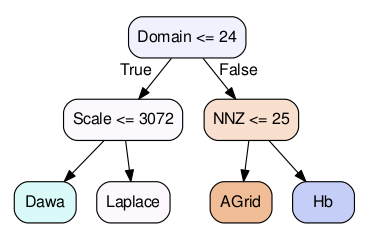
\includegraphics[scale=0.5]{PythiaDTree}
\end{center}
\caption{Example Decision Tree trained by Pythia with features in branches and algorithms in leaves.}\label{fig:pythia}
\end{wrapfigure}
On the other hand, the framework developed in~\cite{Ligett:2017} puts accuracy first. The programmer decides when accuracy is sufficiently high, and privacy usage is then minimized. We refer to this method as NAB since it depends on NoisyAboveThreshold. Critical to the framework is the method of picking correlated Laplacian noise described in~\cite{Koufogiannis:2015}. In this version of the Laplace mechanism, a programmer selects a set of increasing $\epsilon$ values, $(\epsilon_1, \epsilon_2, \ldots, \epsilon_T)$, corresponding to the different budgets they want to try. Correlated Laplace variables $(v_1, v_2, \ldots, v_T)$ are then generated such that knowing a prefix $(v_1, v_2, \ldots, v_t)$ is $\epsilon_t$-differentially private and the noise present in $v_t$ is similar to the noise that a standard Laplace mechanism would add. The framework in~\cite{Ligett:2017} uses this algorithm to add noise to models $m_1, m_2, \ldots, m_T$ when the sensitivities of the models are known. For instance, if the task is linear regression, then the describing a way to iterate through the $v_i$'s until a suitably accurate algorithm is selected. Accuracy can be specified by the programmer as an arbitrary function that takes in a $v_i$. Of course, the release of the most-accurate algorithm has to be done in a differentially-private manner as well, and Ligett et. al use an adaptation of the AboveThreshold algorithm~\cite{Dwork:2006}. This results in an additional privacy and accuracy penalty over simply using the Laplace mechanism with a fixed $\epsilon$. Specifically, if $v_t$ is chosen, then the computation is $\epsilon_t+\epsilon_{Above}$-DP.

Possibly more papers to talk about:~\cite{Winograd-Cort:2017},~\cite{Liu:2018},~\cite{Hsu:2014}.

\chapter{Solution Overview}\label{ch:solution}
\Jostle{} is a differentially-private programming language that introduces a new construct, the \t{ChoiceMaker}. This construct automatically performs meta-machine learning on algorithm input and output pairs and attempts to learn the best-performing algorithm given a private database. This general construct is the first of its kind to automate the process of DP algorithmic choice which normally burdens the programmer. Critical to the success of \Jostle{} is the metafeature, a snapshot of a database, because learning functions from the space of all databases is an intractable problem as the space of databases is large, has little structure, and wouldn't be private. Instead, databases are reduced to their metafeatures, and functions on the metafeature space are learned instead.

First, we present a motivating example for \Jostle{} and then go into a formal description of how the language works. Finally, we discuss what we believe our advantages are over existing solutions.
\section{Motivating Example}
Suppose a programmer is writing code that involves training a decision tree. They may be unsure of which of three decision tree implementations to choose for a decision tree classification problem. A representation of the possible executions of their code is in Figure~\ref{fig:dtree_choices}. The main insight of \Jostle{} is that any time a programmer has an uncertainty, he can write a \t{ChoiceMaker} relatively easily. A \t{ChoiceMaker} works by doing meta-machine learning on traces of the algorithms with labeled input and output pairs and will automatically make the choice. In our example, three linear regressions will be fitted with public information for a database as inputs and the score function of each decision tree algorithm as outputs. We now discuss the formal specification of the \t{ChoiceMaker}.

\begin{figure}
\begin{minipage}{0.5\textwidth}
\begin{center}
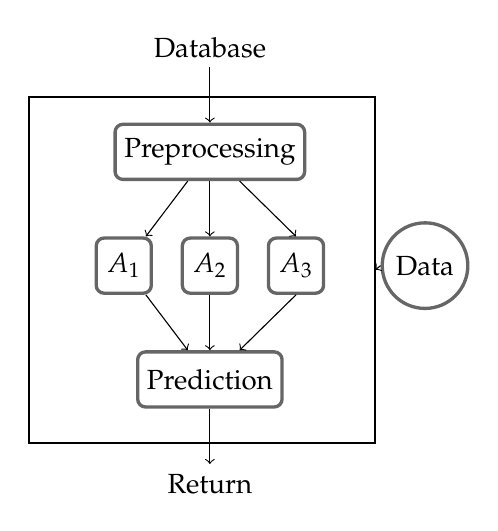
\begin{tikzpicture}[
squarednode/.style={rectangle, draw=black!60, very thick, minimum size=7mm, rounded corners=1mm},
roundnode/.style={circle, draw=black!60, very thick, minimum size=7mm}
]
\node[squarednode] (A) {Preprocessing};
\node (In) [above=2em of A] {Database};
\node[squarednode] (B2) [below=2em of A]{$A_2$};
\node[squarednode] (B1) [left=1em of B2]{$A_1$};
\node[squarednode] (B3) [right=1em of B2]{$A_3$};
\node[squarednode] (C)  [below=2em of B2]{Prediction};
\node (Out) [below=2em of C] {Return};
\node[roundnode] (D) [right=2em of B3]{Data};
\draw[->] (A) -- (B1);
\draw[->] (A.south) -- (B2.north);
\draw[->] (A) -- (B3.north);

\draw[->] (B1) -- (C);
\draw[->] (B2.south) -- (C.north);
\draw[->] (B3.south) -- (C);

%\draw[->] (C.west) .. controls+(left:2em) and +(left:2em) .. (A.west);
\draw[thick] (-2.3,0.7) rectangle(2.1,-3.7);
\draw[->] (D.west) -- (2.1, -1.5);
\draw[->] (In) -- (A);
\draw[->] (C) -- (Out);
\end{tikzpicture}
\end{center}
\end{minipage}
\begin{minipage}{0.5\textwidth}
\begin{lstlisting}[style=MyPythonStyle]
def get_preds(D, eps, test_set):
    D = Preprocess(D, eps*0.3)
    DTreeCM = 
    MkChoiceMaker(
                  public(D),
                  score,
                  dset, 
                  LinReg){
        Alg1, Alg2, Alg3
    }
    model = DTreeCM(D, eps*0.7)
    return model.predict(test_set)
\end{lstlisting}
\end{minipage}
\caption{A motivating example for \Jostle{}. A programmer may be unsure about an execution path (left side), and instead writes a \t{ChoiceMaker} to decide (right side). The metafeatures of this problem are public parts of a database such as the number of columns, domain size (Line 5).}\label{fig:dtree_choices}
\end{figure}
\section{Formal Description}
Let the database space be $\mathcal{R}$, the metafeature space be $\mathcal{X}$, and the answer space be $\mathcal{M}$. $\mathcal{X}$ includes a private database as well as public information such as the number of columns in the database. Any argument passed to the algorithms is also included in $\mathcal{R}$, for example, 2D histogram queries to answer. \Jostle{} uses aggregations and database splits much like PINQ. More capabilities are possible as well as long as any time private data is touched, $\epsilon$ is specified. Additionally, \Jostle{} introduces the \t{Metafeatures}, \t{Option}, and \t{Score} types, and implements constructors with the following types:

\begin{center}
\begin{tabular}{|l|p{7cm}|}
\hline
Name & Type \\ \hline
\t{Metafeatures} & $\mathcal{R} \rightarrow \mathcal{X}$ \\ \hline
\t{MkMetafeatures} & $(\mathcal{R} \rightarrow x_i) \t{ list} \rightarrow \t{Metafeatures}$ \\ \hline
\t{Option} & $\mathcal{R} \rightarrow \mathcal{M}$ \\ \hline
\t{MkOption} & $\mathcal{R} \rightarrow \mathcal{M} \rightarrow \t{Option}$ \\ \hline
\t{Score} & $\mathcal{M}\times\mathcal{R} \rightarrow \mathbb{R}$ \\ \hline
\t{MkScore} & $\mathcal{M}\times\mathcal{R} \rightarrow \mathbb{R} \rightarrow \t{Score}$ \\ \hline
\t{Model} & $\mathcal{X} \rightarrow \mathbb{R}$ \\ \hline
\t{MkModel} & $(\mathcal{X} \times \mathbb{R}) \t{ list} \rightarrow \t{Model} $\\ \hline
\t{ChoiceMaker} & $\mathcal{R} \rightarrow \mathcal{M}$ \\ \hline
\t{MkChoiceMaker} & $\t{Option list} \times \t{Metafeatures}\times \mathcal{R} \t{ list} \times \t{TrainModel} \times \t{Score} \rightarrow \t{ChoiceMaker}$ \\ \hline
\end{tabular}
\end{center}
The functions of each type and the constructors are listed below:
\begin{itemize}
\item{\t{Metafeatures}} Created by \t{MkMetafeatures} which takes in a list of functions $f_1,f_2,\ldots,f_n$ where $f_i$ has type $\mathcal{R} \rightarrow x_i$. These are the metafeature-generating functions. The metafeature space is then $\mathcal{X} = \prod_{i=1}^n x_i$. \t{MkMetafeatures} will return a function that applies all $f_i$'s to a database and return the product.
\item{\t{Option}} Created by \t{MkOption} which takes in the implementation of the algorithm that the \t{Option} represents.
\item{\t{Score}} Created by \t{MkScore} which takes in the score function. The score function tells us, given an answer and possibly using the database, how well the answer did. Usually, the score will be model performance on a validation set.
\item{\t{Model}} Created by \t{MkModel}. This is the model which will learn a function from the metafeatures to the expected algorithm performance. A programmer could greatly change the performance of \Jostle{} by specifying different models, and different algorithmic insights could be revealed.
\item{\t{MkChoiceMaker}} Creates a \t{ChoiceMaker}. This constructor is the most complicated, and its implementation is shown in Figure \ref{fig:choicemaker}. First, models for all the inputted \t{Options} are trained. Then, a function returning the highest \t{Option} for an inputted database is returned. This function is the \t{ChoiceMaker}.
\end{itemize}

\begin{figure}
\begin{lstlisting}[style=MyPythonStyle]
def MkChoiceMaker(ops, feats, train_dbs, mkmodel, score):
    models = []
    for op in ops:
        xypairs = [(feats(db), score(db, op(db))) for db in train_dbs]
        models.append(mkmodel(xypairs))

    def GetAlg(db):
        feat = feats(db)
        perfs = [m(feat) for m in models]
        i = idxmax(perfs)
        return ops[i]
    return GetAlg
\end{lstlisting}
\caption{The implementation of \t{MkChoiceMaker}. }\label{fig:choicemaker}
\end{figure}

\section{Challenges}
Due to the inherent difficulty of performing automatic algorithmic choice as well as its meta-learning design, \Jostle{} presents a unique set of challenges and difficulties over other methods. First, no theoretical guarantees are able to be made about the performance of the \t{NoisyConditional} without further assumptions unlike existing frameworks. This isn't a large problem as algorithmic choice is often solved empirically due to the highly-complex relationships of data-dependent algorithms~\cite{Hay:2016}. More seriously, \Jostle{}'s optimization is limited by the programmer's metafeatures and train databases. If poor metafeatures are inputted or if the public database set is not expansive enough, then the model will almost certainly be impoverished, and the programmer must work to improve it. Luckily, a poor model can be detected after training but before any budget is actually used. We conclude that \Jostle{} removes some of the burden of algorithmic choice from the programmer, but the burden of making a successful model still remains. This is part of the larger problem that doing learning on databases is rather intractable because of the exponential size of the database space; the generality of the \t{ChoiceMaker} forces a difficult learning task.

\section{Advantages}
We believe \Jostle{} exhibits generality that has never been explored by previous approaches. In comparison to existing algorithm frameworks, \Jostle{} makes no assumptions about the score function or the algorithms. Second, \Jostle{} is a programming language that can be represented  We go into more detail about the two types of generality below.

\subsection{Assumption-less choices}
Three existing methods for algorithmic choice \cite{Chaudhuri:2013} \cite{Ligett:2017} \cite{Kotsogiannis:2017}  were discussed on page \pageref{sec:algchoice}. Two of these mechanisms require the sensitivity of the score function to be known, which may not always hold. Some error functions have sensitivities that have pessimistic or even infinite. For example, a viable score function to use on decision trees is the number of correctly classified points in the decision tree. Changing one point in the training set of a decision tree may alter the prediction of a leaf and might alter any number of the predictions for points in the validation set. Thus, the worse-case sensitivity of this function is the size of the database even though one point usually won't change the tree structure at all. Thus, these mechanisms will provide poorer performance than \Jostle{}. The third framework \cite{Kotsogiannis} assumes the 

\subsection{Generality as a Programming Language}
Pythia \cite{Kotsogiannis:2017} is a framework for producing decision trees predicting algorithm selection based on programmer-specified metafeatures. However, one is better off using \Jostle{} every time algorithmic choice is being made rather than instantiating the Pythia framework. \Jostle{} is capable of expressing the entire Pythia framework as a program; indeed, \ref{fig:1} shows one application of the Pythia framework written in \Jostle{}. Repeated uses of algorithmic choice can be succinctly expressed in \Jostle{} rather than Pythia.

\chapter{Experiments and Implementation}\label{ch:experiments}
We demonstrate the functionality and performance of the \Jostle{} code written in Chapter \ref{ch:solution}. The private decision tree literature provides a good opportunity for making algorithmic choice, and there has yet to be a framework developed for them. Our experiments show that the \Jostle{} decision tree code provides an easy and high-performing framework for this. We begin with a preliminary section on Decision Trees and then discuss our experimental setup and results.

\section{Introduction to Private Decision Trees}\label{sec:pdtrees}
In this section, define decision trees, and then we discuss different choices that can make when designing public decision tree algorithms. For each choice, we discuss the additional challenges that arise when making these algorithms private.

\subsection{Decision Tree Preliminaries}
Decision Trees are a powerful tool for data mining due to their high human interpretability, non-parametric design, low computational cost, ability to discover non-linear relationships among attributes, resilience to missing values, ability to handle both discrete and continuous data, and ability to handle non-binary labels~\cite{Fletcher:2016}. Throughout this section, we assume we have a database $D$ with $k$ columns. Suppose the $i$th column can take values in $\mathcal{A}_i$. We call $\mathcal{A}_i$ the attributes of column $i$. Let $c$ be the output column, or ``class'', which we are trying to predict which takes values in $\mathcal{C}$. We assume for simplicity that the $\mathcal{A}_i$ and $\mathcal{C}$ are discrete sets. A decision tree classifies points by branching on attribute $i$, forming $|\mathcal{A}_i|$ subtrees. Once certain criteria are met, no more branching occurs, and instead a leaf node predicts the class. An example Decision Tree is given in Figure~\ref{fig:dt}.

\begin{figure}
\begin{center}
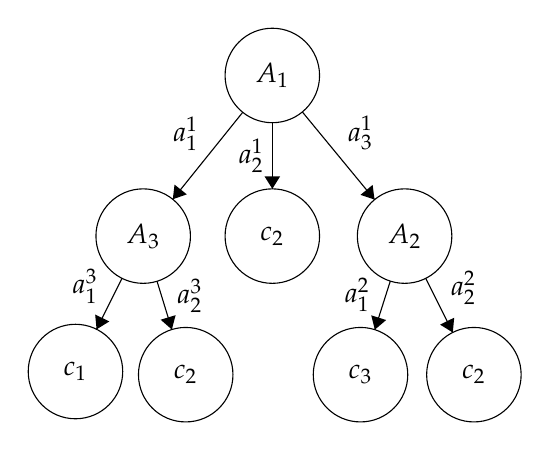
\begin{tikzpicture}[scale=0.2]
\tikzstyle{every node}+=[inner sep=0pt]
\draw [black] (18.1,-4.4) circle (3);
\draw (18.1,-4.4) node {$A_1$};
\draw [black] (9.9,-14.6) circle (3);
\draw (9.9,-14.6) node {$A_3$};
\draw [black] (5.6,-23.2) circle (3);
\draw (5.6,-23.2) node {$c_1$};
\draw [black] (12.6,-23.4) circle (3);
\draw (12.6,-23.4) node {$c_2$};
\draw [black] (18.1,-14.6) circle (3);
\draw (18.1,-14.6) node {$c_2$};
\draw [black] (26.5,-14.6) circle (3);
\draw (26.5,-14.6) node {$A_2$};
\draw [black] (23.7,-23.4) circle (3);
\draw (23.7,-23.4) node {$c_3$};
\draw [black] (30.9,-23.4) circle (3);
\draw (30.9,-23.4) node {$c_2$};
\draw [black] (16.22,-6.74) -- (11.78,-12.26);
\fill [black] (11.78,-12.26) -- (12.67,-11.95) -- (11.89,-11.33);
\draw (13.44,-8.08) node [left] {$a_1^1$};
\draw [black] (18.1,-7.4) -- (18.1,-11.6);
\fill [black] (18.1,-11.6) -- (18.6,-10.8) -- (17.6,-10.8);
\draw (17.6,-9.5) node [left] {$a_2^1$};
\draw [black] (20.01,-6.72) -- (24.59,-12.28);
\fill [black] (24.59,-12.28) -- (24.47,-11.35) -- (23.7,-11.98);
\draw (22.86,-8.07) node [right] {$a_3^1$};
\draw [black] (8.56,-17.28) -- (6.94,-20.52);
\fill [black] (6.94,-20.52) -- (7.75,-20.02) -- (6.85,-19.58);
\draw (7.05,-17.79) node [left] {$a_1^3$};
\draw [black] (10.78,-17.47) -- (11.72,-20.53);
\fill [black] (11.72,-20.53) -- (11.96,-19.62) -- (11.01,-19.91);
\draw (12.02,-18.37) node [right] {$a_2^3$};
\draw [black] (25.59,-17.46) -- (24.61,-20.54);
\fill [black] (24.61,-20.54) -- (25.33,-19.93) -- (24.38,-19.63);
\draw (24.33,-18.34) node [left] {$a_1^2$};
\draw [black] (27.84,-17.28) -- (29.56,-20.72);
\fill [black] (29.56,-20.72) -- (29.65,-19.78) -- (28.75,-20.22);
\draw (29.4,-17.89) node [right] {$a_2^2$};
\end{tikzpicture}
\caption{Example Decision Tree.}\label{fig:dt}
\end{center}
\end{figure}

Decision Trees are made recursively. First, attribute $i$ is chosen, and $D$ is partitioned into groups, one group for each element in $\mathcal{A}_i$. Then, the algorithm is recursively called on each subgroup. When some stopping criteria is met, such as a maximum depth being reached, a leaf is returned which contains some prediction in $\mathcal{C}$. Sometimes, many decision trees are made, and these predictions are aggregated by taking a vote. The general algorithm appears in Figure~\ref{fig:c45}.

The $\mathcal{A}_i$, $\mathcal{C}$, and $k$ are public information. Also, the budget used by recursive calls at the same recursive depth are disjoint. Thus, the total budget usage is
\[
\sum_{i=0}^k \max_{n \in \t{Nodes }n \t{on lvl }i} \epsilon_n
\]
where $\epsilon_n$ is the budget used on node $n$. It makes sense to use the same amount of budget for nodes on the same level, so this simplifies to $\sum_{i=0}^k \epsilon_{k}$.

There are three places that are unspecified in this general algorithm: The conditional that determines whether we stop growing the tree or not (Line 2, stopping criteria), the splitting column for each node (Line 7, greedy choice), and the number of trees in the forest (Line 14, number of trees). These choices are described below.
\begin{figure}

\lstinputlisting[style=MyPythonStyle, firstline=1, lastline=16]{./DTree.py}
\caption{Template for a decision tree algorithm. At Lines 2, 7, and 14, algorithmic choice can be made that change the performance.}\label{fig:c45}
\end{figure}

\subsection{Greedy Choice}
The way in which we choose the column on which to branch is a choice that exhibits data-dependence. Equivalently, we can view the problem as picking the attribute that maximizes the reduction in a potential function. The three choices we consider the Conditional Entropy, Gini coefficient, and the Max Operator~\cite{Friedman:2010}. To describe them, we use the following notation:
We denote by $\tau^{(i)}_{x}$ to be the number of elements of $D$ which have attribute $j$ on column $i$ and $\tau^{(i)}_{x,y}$ to be the number of elements which have attribute $j$ and on column $i$ and class $y$.
Then, the three values are:
\begin{align}
H_i(D) &= \sum_{j\in \mathcal{A}_i}\sum_{c \in \mathcal{C}} {\tau^{(i)}_{j,c}}\ln\left(\frac{\tau^{(i)}_{j}}{\tau^{(i)}_{j,c}}\right) \label{eq:ent} \\
G_i(D) &= \sum_{j \in \mathcal{A}_i} \tau^{(i)}_j\left(1-\sum_{c \in C}\left(\frac{\tau^{(i)}_{j,c}}{\tau^{(i)}_{j}}\right)^2\right)\label{eq:gini} \\
M_i(D) &= \sum_{j \in \mathcal{A}_i} \max_c(\tau^{(i)}_{j,c})
\label{eq:max}
\end{align}

Conditional entropy is the most widely-used potential function in practice, but in the private version, sensitivity comes into play. The sensitivities of the functions are described in the table below:
\begin{center}
\begin{tabular}{|l|l|}
\hline
Name & Sensitivity \\ \hline
Conditional Entropy & $\log(N+1) + \frac{1}{\ln(2)}$ \\ \hline
Gini Index & 2 \\ \hline
Max Opertator & 1 \\ \hline
\end{tabular}
\end{center}
Because the latter two functions have lower sensitivities, less noise must be added to them to make them $\epsilon$-DP per the exponential mechanism. For example, suppose we are choosing between columns $i$, $j$, and $k$ with scores $(3,2,-1)$ for some scoring function. Suppose that the scores under $H_i$ are $(3.1, 1.9, -1.1)$ and that the scores under $G_i$ are $(2.7, 2.2, -0.5)$. Even though $H_i$ is closer in value to the scoring function, its sensitivity is higher. If we have 100 database rows, the sensitivity of $H_i$ is 4.6 compared to 2 for $G_i$. Under 2-DP, the exponential mechanism releases $(i,j,k)$ with probability $(0.46, 0.35, 0.19)$ under $H_i$ and with probability $(0.5, 0.39, 0.11)$ under $G_i$. The expected score of the released answer is 1.9 for $H_i$ and 2.2 for $G_i$. This is an example of how high sensitivity can kill the accuracy of a function when $\epsilon$ is somewhat low.

One last important choice stems from the non-private machine learning literature: picking a random column. This results in less budget expenditure but obviously may lead to poor results. For this reason, random column selection is often combined with multiple trees~\cite{Jagannathan:2009}.

\subsection{Stopping Criteria}
The stopping criteria, or deciding when to make a leaf rather than branch, is another data-dependent choice. Stopping criteria are important to avoid overfitting when there isn't sufficient data in the branch. Having small amounts of data is also susceptible to the noise that DP adds, as relative error goes way up. There are a number of methods in the literature for deciding when to stop~\cite{Fletcher:2016}, and they can be classified into methods that don't use budget and methods that do.
\paragraph{No Budget Use} Without using budget, a ``global'' maximum depth must be used because the data can never be looked at. Maximum depth is a quantity that specifies the maximum recursion depth, or number of branches allowed to be taken before a leaf must be returned. This quantity can be user-specified or based on public information from the database, and we discuss the latter method. Borrowing from rules-of-thumb from non-private data mining, one method is $\frac{k}{2}$ where $k$ is the number of columns in the database. Another method which needs only the size of the initial database $|D|$ is to estimate the branching factor of the decision tree
\[
b = \frac{1}{k}\sum_{i=1}^k|\mathcal{A}_i|
\]
and then to set depth to be $\log_b(D)-1$.
\paragraph{Budget Use} This method queries the database at each branch. The noisy size $n$ of the database is computed privately, and the node is turned into a leaf if
\[
\frac{|D|}{t|C|} < \frac{\sqrt{2}}{\epsilon}
\]
where $t = \max_{i=1}^n|A_i|$. The LHS is an estimation of the signal, or number of points, that a leaf would calculate in each class. If the signal is less than $\frac{\sqrt{2}}{\epsilon}$, the variance of the Laplace distribution, then the calculation stops.

\subsection{Number of Trees}
A random decision forest can drastically outperform a single decision tree~\cite{Fletcher:2016}, and the number of trees in the forest is a data-dependent question. Uniquely in the private setting, if we train $\tau$ trees, we must use $\frac{\beta}{\tau}$ budget for each tree as the trees work on the same dataset. Thus, the number of trees can improve results, but too many trees will harm tree accuracy too much. Also, it even makes sense to have forests for private greedy trees as private trees are inherently random. To ensure tree diversity, it is often forced that each column appear as a member of the first branch an equal number of times, so each column appears approximately $\frac{\tau}{k}$ times in a first branch total.

Once all algorithmic choice has been made and a leaf has been returned, a noisy max over the class counts with the remaining budget is predicted.
Five instantiations of our general decision tree algorithm proposed by other authors are described in Figure \ref{fig:algtable} along with their budgets at each step.

\begin{figure}
\begin{center}
\begin{tabular}{|p{2cm}|p{3cm}|l|p{3cm}|l|p{1cm}|}
\hline
Paper & Stopping Criteria (Line 2) & $\epsilon_{stop}$ & Non-Leaf-Queries (Line 7) & $\epsilon_{NLQ}$ & $\tau$ (L.10) \\ \hline
Friedman \& Schuster~\cite{Friedman:2010} & $d$ user-defined; stop if $\frac{|D|}{t*|C|} < \frac{\sqrt{2}}{\epsilon_{\t{stop}}}$ & $\frac{\beta}{2d}$ & exp. mech with entropy& $\frac{\beta}{2d}$ & 1 \\ \hline
Mohammed et al.~\cite{Mohammed:2015} & $d$ user-defined & 0 & exp. mech with entropy & $\frac{\beta}{d}$ & 1 \\ \hline
Jagannathan et al.~\cite{Jagannathan:2009}, Fletcher \& Islam~\cite{Fletcher:2015} & $d=$ min of $\frac{k}{2}$ and $\log_b(|D|)-1$ & 0 & random & 0 & $\sim 10$ \\ \hline
\end{tabular}
\end{center}
\caption{Instantiations of the algorithm in Figure~\ref{fig:c45}. The total budget is $\beta$. The variable $d$ is the maximum depth that each algorithm uses to compute the budgets at each step.}\label{fig:algtable}
\end{figure}

\section{Experimental Setup and Hypotheses}
The NoisyConditionals we tested are those written in Chapter \ref{ch:solution}. A NoisyConditional is supplied choices, training databases, metafeatures, and models; we give details and justification below.
\paragraph{Choices} We consider only the three decision tree algorithms outlined in Figure \ref{fig:algtable} which we call Algorithms 1, 2, and 3. In Algorithm 1, we set the maximum depth to be 5 always, though the maximum height is rarely reached in most cases because of the additional stopping criteria. In Algorithm 2, we set the maximum height depending on the database size and branching factor in the same way as Algorithm 3, as we believe this is a good rule of thumb. We include three versions of Algorithm 3 with 1, 3, and 7 trees in a forest. We believe choosing among these five algorithms is a complex problem that involves both parameter optimization as well as a diverse set of algorithms.
\paragraph{Training Databases}
Our databases consist of four large, real-world databases with discrete values. Their specifications are included in Figure~\ref{fig:dbinfo}. To obtain more database coverage, we included subsets of this database: We sampled 20, 40, 60, 80, and 100\% of the points and cut off 0, 25, 50, and 75\% of the columns at random, repeating for each pair of values 3 times each except for $(100\%, 0\%)$ as this has no randomness. This results in 58 unique databases made from each real-world database. This results in 232 databases on which we collected algorithm information. For each run of each algorithm, we split the database into 70\% training, trained the algorithm 10 times, then computed the average score on the 30\% validation set.

\paragraph{Metafeatures} We use the following metafeatures: Log of number of rows in the database $\log_{10}(|D|)$, log of the product of the domain size $\log_{10}\left(\prod_{i=1}^k|\mathcal{A}_i|\right)$, the log of the number of classes $\log_{10}(|C|)$, epislon, and the \emph{disuniformity}. We highlighted the importance of the first three values in Section \ref{sec:pdtrees}.

\paragraph{Model} 
The first model we used was regular decision trees  We trained our model on the Protease Cleavage, Nursery, and Tic-tac-toe databases, and used 10 different values of $\epsilon$ from 0.5 to 9. This produced $3\times 58 \times 10$ data points in total. and we pretended that the Loan databases were private and tested our models on these 58 databases. When testing, computing the disuniformity and number of rows takes some of our budget. We decided to allot
\begin{figure}
\begin{center}
\begin{tabular}{|p{3cm}|l|l|l|l|}
\hline
Name & No. Points & No. Cols & Avg. Branch Size & Class size \\ \hline
Protease C & 1625 & 8 & 20 & 2 \\ \hline
Nursery & 12960 & 8 & 3.375 & 5 \\ \hline
Tic-tac-toe & 958 & 9 & 3 & 2 \\ \hline
Student Loan & 1000 & 8 & 6.125 & 2 \\ \hline
\end{tabular}
\end{center}
\caption{Specifications of the four real-world databases used for training.}\label{fig:dbinfo}
\end{figure}

We evaluate \Jostle{} by estimating its regret, or the error relative to the highest-performing algorithm in hindsight, averaged over all databases in the test set.

Our hypotheses are the following:
\begin{itemize}
\item \Jostle{}'s regret will be lower than any individual algorithm, regardless of model and will demonstrate its ability to choose algorithms and tune hyperparameters.
\item \Jostle{}'s trained model will reveal the important metafeatures when making the choice.
\end{itemize}
\section{Results}

\begin{figure}
\begin{center}
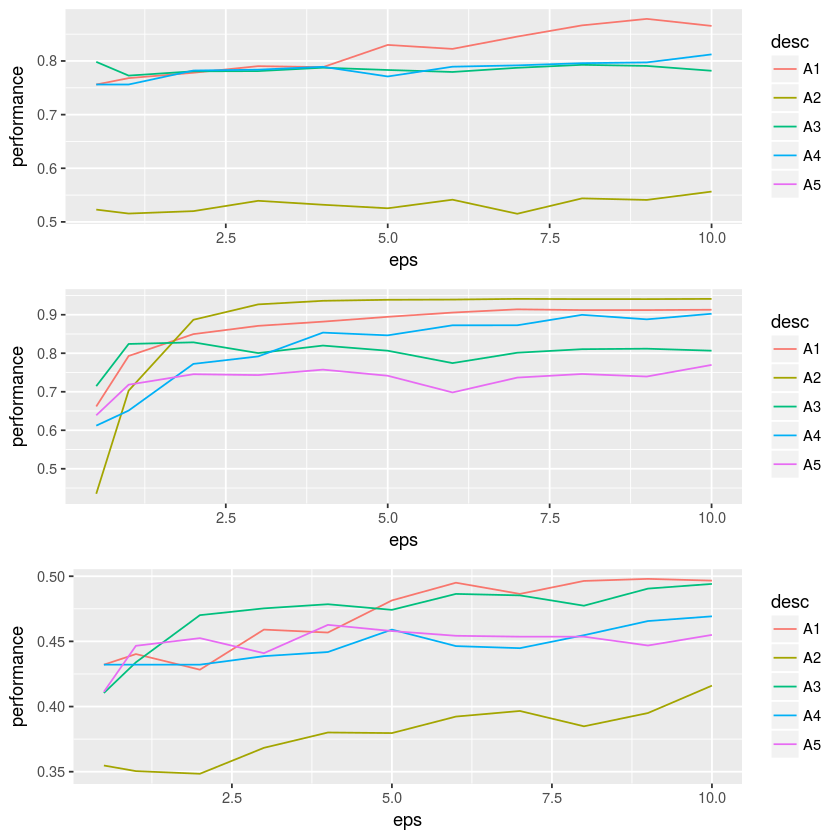
\includegraphics[scale=0.7]{Graph_Performances}
\end{center}
\caption{Performances of the five decision tree algorithms. The performance is measured from the prediction success rate on a validation set using a 30/70 validation to training split. Graph 1 does not have A5 because it takes such a long time to train, having a weak stopping criterion.}
\label{fig:datadep}
\end{figure}

In light of these experiments, we notice that stopping criteria, non-leaf-queries, and the number of trees in the forest have a huge impact on the performance of the algorithm. What a programmer would really like to do is shed light on these complicated relationships in an automated way. It would be easy for her to summarize all of the decision tree algorithms in a chart as in Figure~\ref{alg:dtree}. Each of the two places where she is uncertain is marked with a label, L1 or L2. The goal of \Jostle{} is to learn automatically properties of the database that may lend to a certain decision at L1 or L2.

Our goal is to decide which of the heuristics provided by all the decision trees may perform best, along with any other heuristic the programmer may provide us. 

\chapter{Future Work}\label{ch:future}
We hope to extend \Jostle{} in the following areas: automation, performance optimization, and experiment extent.
\section{Automation}
\Jostle{} places some the burden of finding insights on the programmer via a combination of the \t{Model} and the \t{Metafeatures}. The insights gleamed will only be as powerful as the input metafeatures and any feature-selection done by the \t{Model} during training, so a programmer must still do some analysis before using a \t{ChoiceMaker}. For example, we can observe the metafeatures used in Figure \ref{fig:1} for 2D Histograms.
\begin{lstlisting}[style=MyPythonStyle]
uniformity = Metafeature(data){
    db = data.database
    xgrp = sqrt(db.x_range)
    ygrp = sqrt(db.y_range)
    return {{stddev(select sum(values) from db 
                    groupby x/xgrp, y/ygrp)}}
}
sparsity = Metafeature(data){
    db = data.database
    num_nonzero = {{select count(values) from db 
                    where values > 0}}
    domain_size = db.x_range * db.y_range
    return num_nonzero/domain_size
}
\end{lstlisting}

A programmer would need to have some insights in order to propose these rather-complex metafeatures to a \t{ChoiceMaker}. The analysis contributes to programmer overhead, and perhaps the programmer has made a suboptimal metafeature. To solve this problem, we hope to use algorithm synthesis in the \t{Model} to reduce the complexity of the \t{Metafeatures}. Suppose that, instead of inputting the exact uniformity definition, a programmer indicates the simpler metafeature:
\begin{lstlisting}[style=MyPythonStyle]
uniformity = Metafeature(data){
    db = data.database
    xgrp = sqrt(db.x_range)
    ygrp = sqrt(db.y_range)
    return {{select sum(values) from db 
                    groupby x/xgrp, y/ygrp}}
}
\end{lstlisting}
Instead of returning a real number, an entire database is returned. Instead of learning a regression on the metafeatures, the \t{Model} would learn SQL expressions to aggregate the metafeature databases into a real number. Perhaps it learns that the most suitable aggregation to use is average deviation as opposed to the programmer-specified \t{stddev}. Synthesis can also make edits, too: perhaps instead of using a bucket size of $\sqrt{\t{db.x\_range}}$, a better exponent is $(\t{db.x\_range})^{0.4}$. We find it promising that synthesis for noisy input-output pairs has been done already with deep neural networks \cite{Devlin:2017}, at least when generating a program from scratch as opposed to editing.

\section{Optimization}
\Jostle{} and Pythia both optimize greedily, and there is likely opportunity to greatly improve the performance of \Jostle{}. We say the optimization is greedy because \t{ChoiceMakers} act independently of each other, making the best decisions for themselves but not for the program as a whole. Consider the following juxtaposed \t{ChoiceMakers}:
\begin{lstlisting}[style=MyPythonStyle]
noisyHistChoice = MkChoiceMaker among {DAWA, MWEM}
                    informed by {uniformity, sparsity}
                    trained on trainingSet 
                    wrt ScoreFunc
linRegression = MkChoiceMaker among {LinReg(0.1), LinReg(1)}
                    informed by {size}
                    trained on trainingSet
                    wrt ScoreFunc2
def get_answers(db, y_pts):
    q_answers = noisyHistChoice(db)
    db_mod = modify db using q_answers
    reg_model = linRegression(db_mod)
    return reg_model.predict(y_pts)
\end{lstlisting}
\Jostle{} currently works by optimizing the first and then the second \t{ChoiceMaker}. This is problematic since linRegression depends on an output from noisyHistChoice. The score function of NoisyHistChoice should reflect that it's being fed into linRegression, but it may not and the programmer may not know how to choose the score function. A better way of doing this calculation would be to squish the two \t{ChoiceMakers} together like
\begin{lstlisting}[style=MyPythonStyle]
linRegression = MkChoiceMaker among {(DAWA, LinReg(0.1)),
                                    (MWEM, LinReg(0.1),
                                    (DAWA, LinReg(1)),
                                    (MWEM, LinReg(1))}
\end{lstlisting}
This transformation could be made automatically as an optimization by \Jostle{} and would result in a more globally-optimal algorithm.
\section{Experimental extent}
We would like to do more experiments in the areas of utility functions and hyperparameter optimization. 

Utility functions are used in the exponential mechanism. Some utility functions, like conditional entropy on decision trees, are empirically known to perform the best in the non-private setting. However, in the private setting, an important consideration is the sensitivity of the utility function; if a less-utile function has less sensitivity, then less noise will interfere with its answer. In addition to decision trees, private causal inference exhibits this problem \cite{Kusner:2016}.
\bibliographystyle{plain}
\bibliography{Thesis}
\end{document}